\documentclass{article}

\usepackage{amssymb}
\usepackage{amsmath}
\usepackage{listings}
\usepackage{tikz,pgf}
\usepackage[round]{natbib}

\begin{document}

\title{\huge{A Model for Pre-Cellular RAFs:}  \LARGE{Spontaneous Emergence of Information in Gene--Replicase--Translatase Systems}}
%\author{Alex Popinga, Alexei Drummond, Peter Wills}
\author{Alex Popinga}
\date{\today}
\maketitle

\section{Introduction}
The origin of life on Earth remains a largely mysterious and open problem 
spanning multiple disciplines of science.  Fundamentally, we seek to understand the process of naturally generating polymeric species 
capable of distinguishing themselves from a homogenous, ``noisy" solution by self-replicating with increasing fidelity, efficiency, 
and complexity, i.e., diversity of function \citep{NASA}. %by non-equilibrium phase transitions. \cite{Wills2015} \cite{NASA}

In 1971, preliminary work toward this goal was performed by theoretical biologist and complex systems researcher Stuart Kauffman.  \citet*{Kauffman1971} suggested that ``proto-organisms'' probably arose from chemical reaction systems, 
which he later \citep{Kauffman1986} elaborated as ``reflexively autocatalytic sets of peptides and polypeptides".
In 2000, Steel formalised Kauffman's "connected, reflexively autocatalytic" sets \citep{Steel2000} into RAF (reflexively autocatalytic, food-generated) set theory.
Steel's formalisation was followed by investigations into irreducible RAFs \citep{Steel2013,Hordijk2014}, RAF algorithms with increasing computational efficiency \citep{Hordijk2004,Hordijk2015}, RAFs with inhibitory molecules \citep{Hordijk2012a,Hordijk2015}, and so forth.

We briefly review RAF theory now.

\subsection{RAF theory}
A chemical reaction system (CRS) is defined as a tuple commonly denoted ($X$, $R$, $C$), where $X$ is the set of molecule types, 
$R$ is the set of chemical reactions, and $C$ is the catalytic set that describes which reactions are catalysed by which molecule types. \citep{Hordijk2015}
With the addition of a `food' set $F$, which is a subset of the molecules in $X$ assumed to be limitlessly available in the environment and not necessarily produced by a reaction 
in $R$, the CRS becomes the quadruple $Q = (X, R, C, F)$.  A subset of $R$, $R' \subseteq R$, is a RAF if it satisfies the following conditions:

(1) It is \textit{reflexively autocatalytic} (RA), meaning that every reaction $r \in R'$ is catalysed by either a molecule in the food set $F$ or a molecule produced by one of a series of reactions starting with $F$.

(2) It is \textit{food-generated} (F), meaning that for every reaction in $R'$ the reactant is either in the food set $F$ or can eventually be generated by a series of reactions starting with molecules in $F$.

As described by \cite{Kauffman1986} and as done in previous RAF work \citep{Hordijk2004,Hordijk2015}, we choose a binary polymer model to explore the application of RAF theory to abstractions of information-carrying molecules in prebiotic systems.  

\subsection{Unlike RAF: Error, death, and diffusion}

Unlike in previous RAF work, we add the potential for reactions to occur with `error', or imperfectly, meaning that not only the most desired or the most probable products are yielded 
by reactions in the set $R$.  In other words, at some small rate molecules are produced that are not in the set $X$ and therefore outside of the RAF.   

Additionally, we add two uncatalysed reactions for simulating the processes of degradation (death) and diffusion.  The latter was proposed by \cite{Turing} as part of his reaction-diffusion system.
The reaction-diffusion system is important as it describes how non-uniform patterns can emerge from homogenous states.  This is significant to the pursuit of information-carrying molecules 
emerging from homogenous, `noisy' solutions, including those within RAFs. 

We describe our binary polymer model in detail below.

%\subsection{The Informed Generation}
%The most fundamental theory in biology, that of evolution by natural selection, describes the continual editing of the genetic code into various translations, i.e., phenotypic characteristics.  
%It does not concern itself with the origins of genetic information or mode of emergence.

\section{The Gene-Replicase-Translatase (GRT) Model}

Genes are described as binary sequences of length $L$.  For a small system of $L=3$, the set $G = \{000, 001, 010, 011, \dots, 111\}$ contains 8 possible genes.  An individual gene is denoted $g \in G$. Proteins are also described as binary sequences of length $L$, but we distinguish them by using a unique alphabet such that $P = \{AAA, AAB, ABA, ABB, \dots, BBB\}$, and an individual protein is $p \in P$. 

In this primitive system we imagine a simple translation mechanism in which one `nucleotide' position in a gene is translated to one `amino acid' in a protein.  In other words, a codon is also represented by a single bit, and therefore a gene and its translated protein are always the same length.

The reactions in the set $R$ are:  

\hspace{3mm} ($r0$) gene replication (birth of a gene), 

\hspace{3mm} ($r1$) gene translation (birth of a protein),
 
\hspace{3mm} ($r2$) degradation (death of either a gene or a protein), 

\hspace{3mm} ($r3$) diffusion (movement of either gene or protein into an adjacent `cell').

The corresponding catalysts that describe the set $C$ for these reactions are:

\hspace{3mm} ($r0$) the gene to be replicated, acting as a template, and a replicase protein,

\hspace{3mm} ($r1$) the gene to be translated, as a template, and a translatase protein,

\noindent{(Notice that $r2$ and $r3$ are uncatalysed reactions.  These place our system outside of the strict definition of a RAF.)}
These reactions are shown in Figure 1.

\begin{figure}
\begin{center}
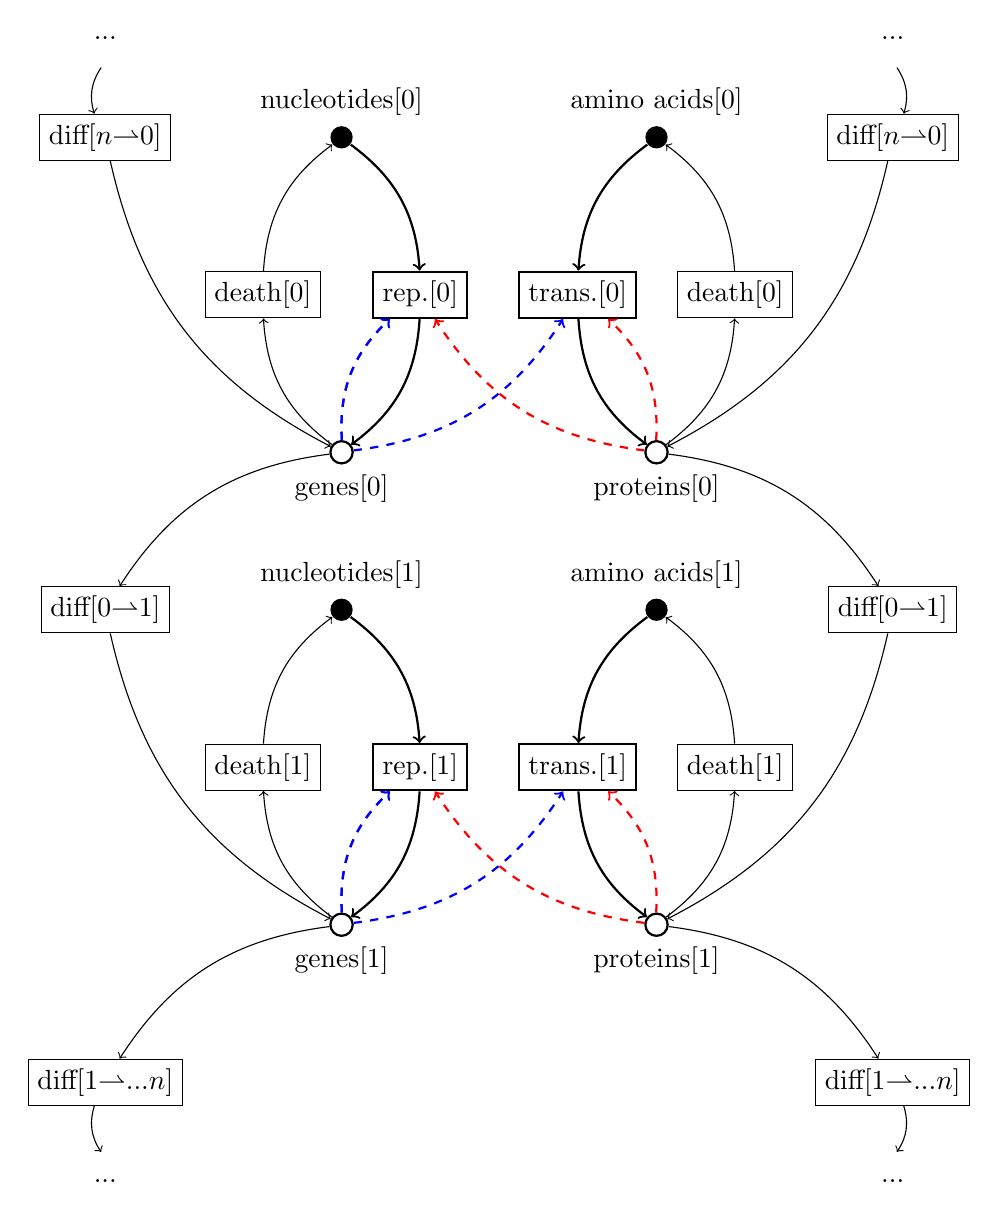
\begin{tikzpicture}

% genes node
\node[thick,circle, draw,inner sep=1mm] (genes) at (-2,0) {};
\node[below] at (genes.south) {genes[0]};

% rep. reaction node
\node[thick,rectangle,draw] (r) at (-1,2) {rep.[0]};

% nucleotides node
\node[circle, fill,inner sep=1mm] (nucleotides) at (-2,4) {};
\node[above] at (nucleotides.north) {nucleotides[0]};

\draw[thick,->] (r) to [bend left=25] (genes);
\draw[thick,dashed,blue,->] (genes) to [bend left=25] (r);
\draw[thick,->] (nucleotides) to [bend left=25] (r);

% proteins node
\node[thick,circle, draw,inner sep=1mm] (proteins) at (2,0) {};
\node[below] at (proteins.south) {proteins[0]};

% trans. reaction node
\node[thick,rectangle,draw] (t) at (1,2) {trans.[0]};

% amino acids node
\node[circle, fill,inner sep=1mm] (amino acids) at (2,4) {};
\node[above] at (amino acids.north) {amino acids[0]};

\draw[thick,->] (amino acids) to [bend right=25] (t);
\draw[thick,->] (t) to [bend right=25] (proteins);

\draw[thick,dashed,red,->] (proteins) to [bend left=25] (r);
\draw[thick,dashed,red,->] (proteins) to [bend right=25] (t);
\draw[thick,dashed,blue,->] (genes) to [bend left=25] (r);
\draw[thick,dashed,blue,->] (genes) to [bend right=25]  (t);

% genes degradation reaction node
\node[rectangle,draw] (genes death) at (-3,2) {death[0]};

% genes diff reaction node
\node[rectangle,draw] (genes diff) at (-5,-2) {diff[0$\rightharpoonup$1]};

% proteins degradation reaction node
\node[rectangle,draw] (proteins death) at (3,2) {death[0]};

% proteins diff reaction node
\node[rectangle,draw] (proteins diff) at (5,-2) {diff[0$\rightharpoonup$1]};

\draw[->] (proteins death) to [bend right=25] (amino acids);
\draw[->] (proteins) to [bend right=25] (proteins death);

\draw[->] (genes death) to [bend left=25] (nucleotides);
\draw[->] (genes) to [bend left=25] (genes death);

\draw[->] (genes) to [bend right=25] (genes diff);
\draw[->] (proteins) to [bend left=25] (proteins diff);

%
% cell 1 nodes...
%
\node[thick,circle, draw,inner sep=1mm] (genes1) at (-2,-6) {};
\node[below] at (genes1.south) {genes[1]};
\node[thick,circle, draw,inner sep=1mm] (proteins1) at (2,-6) {};
\node[below] at (proteins1.south) {proteins[1]};

\draw[->] (genes diff) to [bend right=25] (genes1);
\draw[->] (proteins diff) to [bend left=25] (proteins1);

% rep. reaction node 1
\node[thick,rectangle,draw] (r1) at (-1,-4) {rep.[1]};

% nucleotides node 1
\node[circle, fill,inner sep=1mm] (nucleotides1) at (-2,-2) {};
\node[above] at (nucleotides1.north) {nucleotides[1]};

\draw[thick,->] (r1) to [bend left=25] (genes1);
\draw[thick,dashed,blue,->] (genes1) to [bend left=25] (r1);
\draw[thick,->] (nucleotides1) to [bend left=25] (r1);

% trans. reaction node 1
\node[thick,rectangle,draw] (t1) at (1,-4) {trans.[1]};

% amino acids node 1
\node[circle, fill,inner sep=1mm] (amino acids1) at (2,-2) {};
\node[above] at (amino acids1.north) {amino acids[1]};

\draw[thick,->] (amino acids1) to [bend right=25] (t1);
\draw[thick,->] (t1) to [bend right=25] (proteins1);

\draw[thick,dashed,red,->] (proteins1) to [bend left=25] (r1);
\draw[thick,dashed,red,->] (proteins1) to [bend right=25] (t1);
\draw[thick,dashed,blue,->] (genes1) to [bend left=25] (r1);
\draw[thick,dashed,blue,->] (genes1) to [bend right=25]  (t1);

% genes degradation reaction node 1
\node[rectangle,draw] (genes death1) at (-3,-4) {death[1]};

% proteins degradation reaction node 1
\node[rectangle,draw] (proteins death1) at (3,-4) {death[1]};

\draw[->] (proteins death1) to [bend right=25] (amino acids1);
\draw[->] (proteins1) to [bend right=25] (proteins death1);

\draw[->] (genes death1) to [bend left=25] (nucleotides1);
\draw[->] (genes1) to [bend left=25] (genes death1);

% genes diff reaction node 1
\node[rectangle,draw] (genes diff1) at (-5,-8) {diff[1$\rightharpoonup$...$n$]};

% proteins diff reaction node 1
\node[rectangle,draw] (proteins diff1) at (5,-8) {diff[1$\rightharpoonup$...$n$]};

\draw[->] (genes1) to [bend right=25] (genes diff1);
\draw[->] (proteins1) to [bend left=25] (proteins diff1);

%
% cell (...) nodes...
%
\node[thick,inner sep=1mm] (blah0) at (-5,-9) {};
\node[below] at (blah0.south) {...};
\node[thick,inner sep=1mm] (blah1) at (5,-9) {};
\node[below] at (blah1.south) {...};

\draw[->] (genes diff1) to [bend right=25] (blah0);
\draw[->] (proteins diff1) to [bend left=25] (blah1);

% genes diff reaction node 2
\node[rectangle,draw] (genes diff2) at (-5,4) {diff[$n$$\rightharpoonup$0]};

% proteins diff reaction node 2
\node[rectangle,draw] (proteins diff2) at (5,4) {diff[$n$$\rightharpoonup$0]};

\node[thick,inner sep=1mm] (blah2) at (-5,5) {};
\node[above] at (blah2.north) {...};
\node[thick,inner sep=1mm] (blah3) at (5,5) {};
\node[above] at (blah3.north) {...};

\draw[->] (blah2) to [bend right=25] (genes diff2);
\draw[->] (blah3) to [bend left=25] (proteins diff2);

\draw[->] (genes diff2) to [bend right=25] (genes);
\draw[->] (proteins diff2) to [bend left=25] (proteins);

\end{tikzpicture}
\caption{The circle nodes represent molecule types in the set $X$, while the black circles indicate those specifically within the food set $F$.
The rectangular boxes show the reaction nodes.  Indices are used to assign the `cell', which is simply a location in space where the molecules are and the reactions take place.}
\end{center}
\end{figure}


In this system, all proteins in the set $P$ have varying levels of catalytic activity for replication and translation. A replication reaction, with a gene $g$ acting as template can proceed either without error, such as

\begin{equation}
010 \xrightarrow[]{AAA} 010 + 010\quad \text{ at rate } \alpha_1,
\label{eq:basicRep}
\end{equation}

\noindent{or with error, for example}

\begin{equation}
010 \xrightarrow[]{AAA} 010 + 011\quad \text{ at rate } \alpha_2.
\label{eq:basicError}
\end{equation}

\noindent{(We assume the food set $F = \{0,1\}$ contains an infinite supply of elements ``0" and ``1", the nucleotides, and is an implicit component of the lefthand side of eq.~\ref{eq:basicRep},\ref{eq:basicError}.)}

Translation reactions are modelled in a stepwise fashion so that partial translation yields intermediate complexes that are explicit species in the system: 

\begin{equation}
 \begin{array}{l l}
010 \xrightarrow[]{ABA} \overset{A}010 & \quad \text{ at rate } \beta_1 \\
\\
\overset{A}010 \xrightarrow[]{BAB} \overset{A}0\overset{B}10 & \quad \text{ at rate } \beta_2\\
\\
\overset{A}0\overset{B}10 \xrightarrow[]{ABA} 010 + ABA & \quad \text{ at rate } \beta_3
\end{array}
\label{eq:basicTrans}
\end{equation}

\noindent{Above, $ABA$ is a translatase that is translating the codon `0' to the amino acid `$A$' and $BAB$ is a translatase translating the codon `1' to the amino acid `$B$' at the specified rates.  
As with the replication reactions, translation reactions proceed at higher rates for particular specifications but also have some rate at which an alternative outcome occurs (e.g., $ABA$ translates the codon `0' to the amino acid `$B$' rather than `$A$').}

\subsection{Diffusion representation}

We make a small change of notation to introduce a spatial component for diffusion reactions, where space is described by a linear array of cells indexed by $i$. The replication reaction introduced in eq.~\ref{eq:basicRep} is now represented in cell $i$ as:

\begin{equation}
G_{010}[i] \xrightarrow[]{P_{000}[i]}G_{010}[i] + G_{010}[i]\quad \text{ at rate } \gamma_1,
\end{equation}

\noindent{and now a diffusion reaction from cell $i$ to cell $j$ can also occur, such that:}

\begin{equation}
G_{010}[i] \xrightarrow[]{}G_{010}[j] \quad \text{ at rate } \gamma_2, \text{ with }|i-j|=1.
\end{equation}


\section{A simplified monopolymer model}

To help us understand some of the basic dynamics, and to compare with our full GRT model, we also consider a simplified monopolymer model of length $L=2$. 
Here we assume that both replication and translation reactions occur perfectly, i.e., without error.  %Also, translation reactions occur in a single step, so that no intermediate species are represented in the system. 
%As before, we explicitly describe food sources as nucleotide and amino acid monomers. 
%We therefore have two symmetric replication and translation reactions, 
If a gene is represented as nucleotide polymer $nn$, the catalytic template, and a protein as amino acid polymer $aa$, is the catalytic enzyme, then we have:

\begin{equation}
2n \xrightarrow[nn]{aa} nn\quad \text{replication at rate } \rho,
\label{eq:simplifiedRep}
\end{equation}

\begin{equation}
2a \xrightarrow[nn]{aa} aa\quad \text{translation at rate } \tau.
\label{eq:simplifiedTranslation}
\end{equation}

Again, we introduce two density-dependent degradation rates to prevent the system from growing without bound:

\begin{equation}
nn \xrightarrow[]{nn} 2n\quad \text{gene degradation at rate } \mu_1,
\label{eq:simplifiedRep}
\end{equation}

\begin{equation}
aa \xrightarrow[]{aa} 2a\quad \text{protein degradation at rate } \mu_2.
\label{eq:simplifiedTranslation}
\end{equation}

The change in concentration of the two polymer species ($m=nn$ and $p=aa$) and their two food sources ($a$ and $n$) could be described deterministically by the following system of ordinary differential equations (ODEs):
\begin{align}
\dot{m} &= \rho mpn^2 - \mu_1 m, \\
\dot{p} &= \tau mpa^2 - \mu_2 p, \\
\dot{n} &= 2\mu_1m,\\
\dot{a} &= 2\mu_2p.
\end{align}

Like the full GRT model, this simplified model (depicted in Figure \ref{fig:simplifiedRAF}) is not quite either RAF or pseudo-RAF in Steel's classification, as the death reactions are not catalysed.

\begin{figure}
\begin{center}
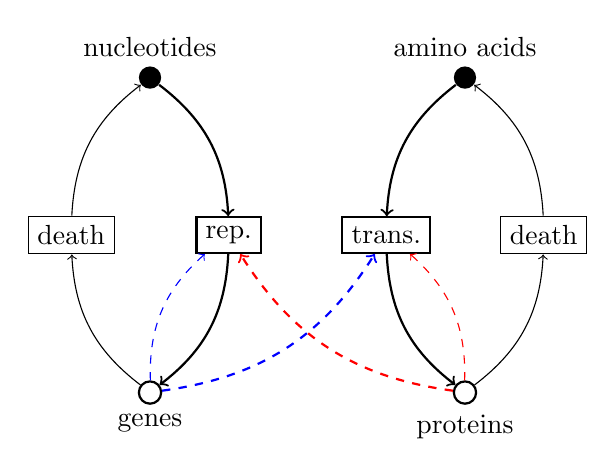
\begin{tikzpicture}

% n node
\node[thick,circle, draw,inner sep=1mm] (genes) at (-1,0) {};
\node[below] at (genes.south) {genes};

% replication reaction node
\node[thick,rectangle,draw] (rep) at (0,2) {rep.};

% nn node
\node[circle, fill,inner sep=1mm] (nucleotides) at (-1,4) {};
\node[above] at (nucleotides.north) {nucleotides};

\draw[thick,->] (nucleotides) to [bend left=25] (rep);
\draw[thick,->] (rep) to [bend left=25] (genes);

% a node
\node[thick,circle, draw,inner sep=1mm] (proteins) at (3,0) {};
\node[below] at (proteins.south) {proteins};

% translation reaction node
\node[thick,rectangle,draw] (trans) at (2,2) {trans.};

% nn node
\node[circle, fill,inner sep=1mm] (amino acids) at (3,4) {};
\node[above] at (amino acids.north) {amino acids};

\draw[thick,->] (amino acids) to [bend right=25] (trans);
\draw[thick,->] (trans) to [bend right=25] (proteins);

\draw[thick,dashed,red,->] (proteins) to [bend left=25] (rep);
\draw[thick,dashed,blue,->] (genes) to [bend right=25]  (trans);

% nucleotide degradation reaction node
\node[rectangle,draw] (death_gene) at (-2,2) {death};

% nucleotide degradation reaction node
\node[rectangle,draw] (death_protein) at (4,2) {death};

\draw[->] (proteins) to [bend right=25] (death_protein);
\draw[->] (death_protein) to [bend right=25] (amino acids);

\draw[->] (genes) to [bend left=25] (death_gene);
\draw[->] (death_gene) to [bend left=25] (nucleotides);

\draw[dashed,red,->] (proteins) to [bend right=25] (trans);
\draw[dashed,blue,->] (genes) to [bend left=25] (rep);

\end{tikzpicture}
\end{center}
\caption{\label{fig:simplifiedRAF} A simplified replication-translation model. The food set $F = \{$nucleotides, amino acids$\}$, and $X = \{$nucleotides, amino acids, genes, proteins$\}$ is the set of molecules.}
\end{figure}


\section{Simulations of stochastic dynamics}

To better investigate the dynamics of the system, we performed Gillepsie simulations in MASTER \citep{MASTER}, a software package for simulating stochastic population dynamics using chemical master equations. 

We added indices to represent the sequence and location of each species.  This allows us to describe all possible reactions for all possible gene and protein species in a single line.  
For example, all replication reactions, as exemplified in eq.~\ref{eq:basicRep}, are now represented as:

\begin{equation}
 \begin{array}{l l}
 G[i1,i2,i3,l1] + P[a1,a2,a3,l1] + SG[l1]\\
 
\xrightarrow[]{} G[i1,i2,i3,l1] + P[a1,a2,a3,l1] + G[j1,j2,j3,l1],\\
\end{array}
\label{eq:masterRep}
\end{equation}

\noindent{with the gene sequence $i1,i2,i3$ being replicated with some small rate of error (akin to mutation) to sequence $j1,j2,j3$.  The index $l1$ denotes the `cell' that contains the species.  
Genes occupy gene space $SG$ within the cell, while proteins occupy protein space $SP$.}
The translation reactions in eq.~\ref{eq:basicTrans} are now represented as:

\begin{equation}
 \begin{array}{l l}
G[i1,i2,i3,l1] + P[a1,a2,a3,l1] + SP[l1] \\

\xrightarrow[]{} GP[i1,i2,i3,e1,l1] + P[a1,a2,a3,l1] \\
\\
GP[i1,i2,i3,e1,l1] + P[a1,a2,a3,l1] \\

\xrightarrow[]{} GP1[i1,i2,i3,e1,e2,l1] + P[a1,a2,a3,l1] \\
\\
GP1[i1,i2,i3,e1,e2,l1] + P[a1,a2,a3,l1] \\

\xrightarrow[]{} G[i1,i2,i3,l1] + P[e1,e2,e3,l1] + P[a1,a2,a3,l1] \\
\end{array}
\label{eq:masterTrans}
\end{equation}

\noindent{with additional indices $e1$ and $e2$ to denote either the `$A$' or `$B$' amino acid forming the partially translated gene-protein complexes $GP$ and $GP1$.}
Each of these reactions has a rate specified within the reaction element.  

MASTER also allows the option of applying a rate multiplier, which can be useful for adjusting the rate at which a particular reaction occurs based off of, for example, Hamming distances.
For the replication reactions we use a Poissonian distributed Hamming distance rate multiplier with mutation rate 0.01.  
The exponential function `exp(-a1-a2-a3)' applies to the proteins catalysing the reaction, with the protein sequence P[0,0,0] as the most effective replicase.  
Together with eq.~\ref{eq:masterRep}, the full reaction element for replication is: 

\lstset{
  basicstyle=\ttfamily,
  columns=fullflexible,
  showstringspaces=false,
  commentstyle=\color{gray}\upshape
}

\lstdefinelanguage{XML}
{
  morestring=[b]",
  morestring=[s]{>}{<},
  morecomment=[s]{<?}{?>},
  stringstyle=\color{black},
  identifierstyle=\color{darkblue},
  keywordstyle=\color{cyan},
  morekeywords={xmlns,version,type}% list your attributes here
}

\footnotesize{
\begin{lstlisting}

<reaction spec='Reaction' reactionName="Replication" rate="1">
    <rateMultiplier spec='RateMultiplier'> 
        exp(-a1-a2-a3)*dpois(HD({i1,i2,i3},{j1,j2,j3}),0.01)
    </rateMultiplier>
        G[i1,i2,i3,l1] + P[a1,a2,a3,l1] + SG[l1] ->  
        G[i1,i2,i3,l1] + P[a1,a2,a3,l1] + G[j1,j2,j3,l1]
</reaction>         
        
\end{lstlisting}}

\normalsize{\noindent{The translation reactions use a look-up `key' to specify the amino acid $e$ 
to be translated from codon $i$ by the protein sequence P[$a1,a2,a3$].  The translations without error proceed as follows:} 

P[0,1,1] translates codon `0' to amino acid `0' (`$A$'), 

P[0,1,0] translates codon `1' to amino acid `1' (`$B$'), 

P[1,0,0] translates codon `0' to amino acid `1' (`$B$'),  

P[0,0,1] translates codon `1' to amino acid `0' (`$A$').  

\noindent{The errors introduced in translation are determined by the exponential function `exp(-HD(key(i1,e1),{a1,a2,a3})/0.1)', 
where `HD' is the Hamming distance and 0.1 is the catalytic width.  Together with eq.~\ref{eq:masterTrans}, the reaction element for translation is:}}

\lstset{
  basicstyle=\ttfamily,
  columns=fullflexible,
  showstringspaces=false,
  commentstyle=\color{gray}\upshape
}

\lstdefinelanguage{XML}
{
  morestring=[b]",
  morestring=[s]{>}{<},
  morecomment=[s]{<?}{?>},
  stringstyle=\color{black},
  identifierstyle=\color{darkblue},
  keywordstyle=\color{cyan},
  morekeywords={xmlns,version,type}% list your attributes here
}

\footnotesize{
\begin{lstlisting}

<reaction spec='Reaction' reactionName="Translation" rate="1">
    <rateMultiplier spec='RateMultiplier' value="exp(-HD(key(i1,e1),{a1,a2,a3})/0.1)"/>
        G[i1,i2,i3,l1] + P[a1,a2,a3,l1] + SP[l1] -> 
        GP1[i1,i2,i3,e1,l1] + P[a1,a2,a3,l1] + G[i1,i2,i3,l1] 
</reaction>          
<reaction spec='Reaction' reactionName="Translation1" rate="9">
    <rateMultiplier spec='RateMultiplier' value="exp(-HD(key(i2,e2),{a1,a2,a3})/0.1)"/>
        GP1[i1,i2,i3,e1,l1] + P[a1,a2,a3,l1] -> 
        GP2[i1,i2,i3,e1,e2,l1] + P[a1,a2,a3,l1]
</reaction>
<reaction spec='Reaction' reactionName="Translation2" rate="9">
    <rateMultiplier spec='RateMultiplier' value="exp(-HD(key(i3,e3),{a1,a2,a3})/0.1)"/>
        GP2[i1,i2,i3,e1,e2,l1] + P[a1,a2,a3,l1] -> 
        P[e1,e2,e3,l1] + P[a1,a2,a3,l1]
</reaction>        
        
\end{lstlisting}}

\normalsize{To add diffusion reactions, a predicate function is used to determine which species will be moved to which location based off of the location indices of the species.  
In the following example, the diffusion space is characterised by an annulus:}

\lstset{
  basicstyle=\ttfamily,
  columns=fullflexible,
  showstringspaces=false,
  commentstyle=\color{gray}\upshape
}

\lstdefinelanguage{XML}
{
  morestring=[b]",
  morestring=[s]{>}{<},
  morecomment=[s]{<?}{?>},
  stringstyle=\color{black},
  identifierstyle=\color{darkblue},
  keywordstyle=\color{cyan},
  morekeywords={xmlns,version,type}% list your attributes here
}

\footnotesize{
\begin{lstlisting}

<reaction spec=`Reaction' reactionName="Diffusion_G" rate="0.01">
    <predicate spec=`Predicate' value="abs(l1-l2)==1 || abs(l1-l2)==G_dim[3]"/>
        G[i1,i2,i3,l1] + SG[l2] -> G[i1,i2,i3,l2] + SG[l1]
</reaction>          
        
\end{lstlisting}}


\section{(Preliminary) simulation results in MASTER}

\normalsize{For the symmetrical monopolymer model, the populations of amino acid and nucleotide food molecules, and the `NN' gene and `AA' protein populations,
quickly reached an equilibrium, as shown in Figure 3.  

This also appeared to be true for the `perfect GRT' model (with 3 binary $L=3$ gene species 
and 3 corresponding binary proteins with $L=3$), which behaves as a RAF in that no error is generated by either the replication or translation reactions. 
(In fact, it should be noted that this first implementation of the minimal GRT model in MASTER is similar to a CAF, a stronger notion of RAF that has a food 
set with molecules - here including genes and proteins along with nucleotides and amino acids - which acts as catalysts immediately in the system.  However, the degradation reactions are uncatalyzed.) 

When only nucleotides and amino acids were initially present in the system (and simulation time was extended), it was observed that one of the 3 gene species quickly stabilized 
while another became predominate and the third went to zero (occasionally being produced in small quantities by random food-generated-only reactions), as shown in Figure 4.

Replacing explicit food molecules (i.e., nucleotide and amino acid species) with spaces - in which the genes occupy a single space $S$, the gene-protein complexes each 
a single space $S$, and the proteins occupy three spaces ($3S$) - caused a similar but distinctive behaviour.  In this case, one of the 3 gene species clearly began to dominate while 
the other two began to die out and that eventually the whole system collapsed (Figure 5).  Increasing the simulation time again showed that all populations 
clearly went to zero.

Figure 6 shows results from the implementation of the minimal GRT model with all 8 gene and all 8 protein species possible (i.e., with error in the replication and translation reactions) in 3 unique cells, but with no diffusion reactions taking place to pass molecules from cell to cell.

Finally, Figure 7 shows preliminary results from the implementation of the full minimal GRT model, with error possible in the replication and translation reactions, and with diffusion among 3 cells described by an annulus (cell 0 to cell 1, cell 1 to cell 2, cell 2 to cell 0).

\subsection{Concluding remarks}

We intend to increase the number of cells and the length of the simulations.  Currently, the computation time required is astronomical, as MASTER was designed to handle large numbers of species types but few reactions.  
Our model has relatively few molecule types, but many reactions (when including all possibilities for error in replication and translation).

That being said, our initial investigations seem to suggest that diffusive processes are important for RAFs that contain reactions that can proceed with error.  This would follow our prediction, as diffusion provides a mechanism for separating molecules that are outside the RAF system so that they do not impede the production of RAF molecules by stealing resources - i.e., reactants and catalysts.
Furthermore, results obtained by \cite{Paoletti}, who ran Gillepsie simulations to study the dynamics of real molecule populations in networks that contain RAFs, seem to agree with our results.
Paoletti found that molecules outside of the RAFs were being generated just as much, if not more, than the molecules within the RAF set $X$.

Further work would be to explore both our model as well as that of Paoletti, the latter of which might prove to show similar behaviour once allowed diffusion.

\begin{figure}
    \centering
    	\quad
    	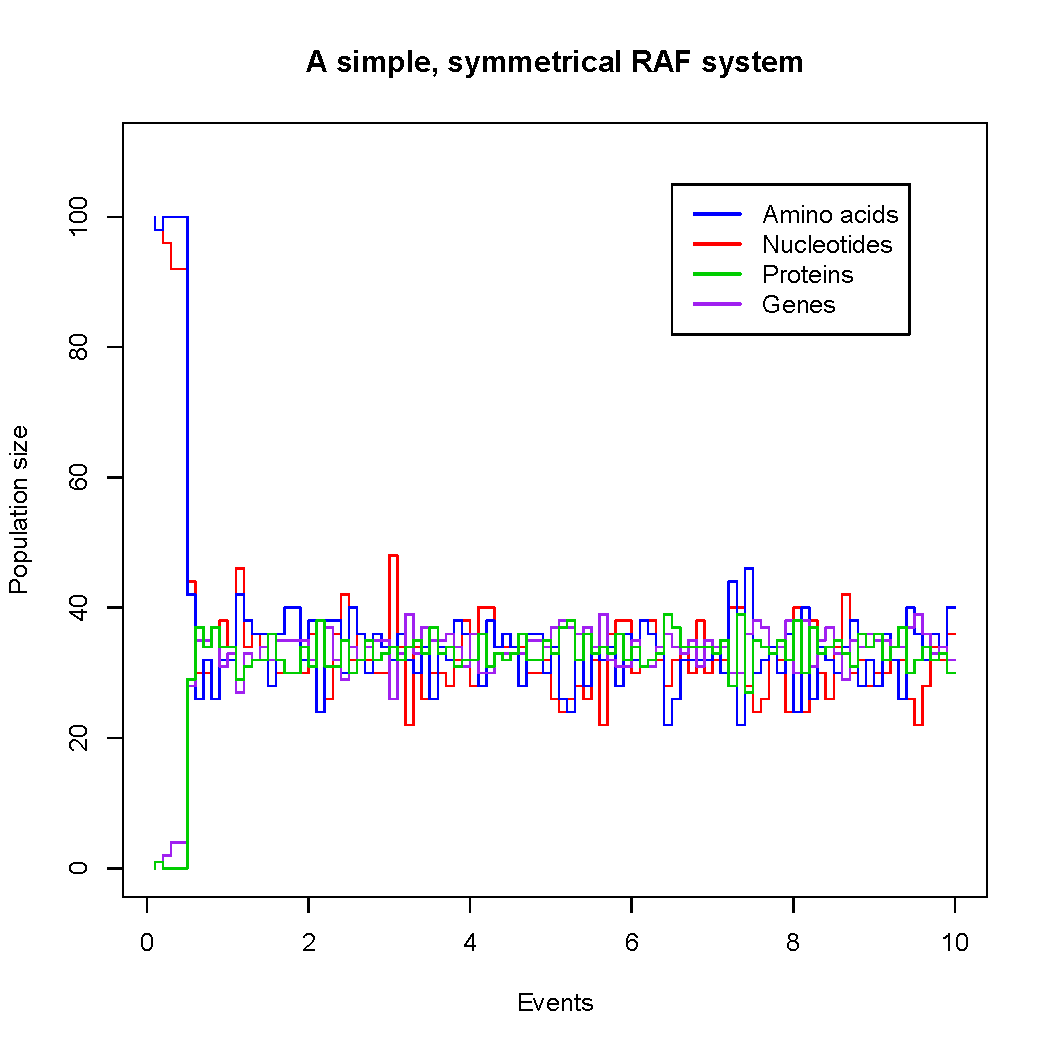
\includegraphics[width=3.5in]{InitiallyOnlyNucAndAAInitiallyUncatalyzed.pdf}
    	\quad
    	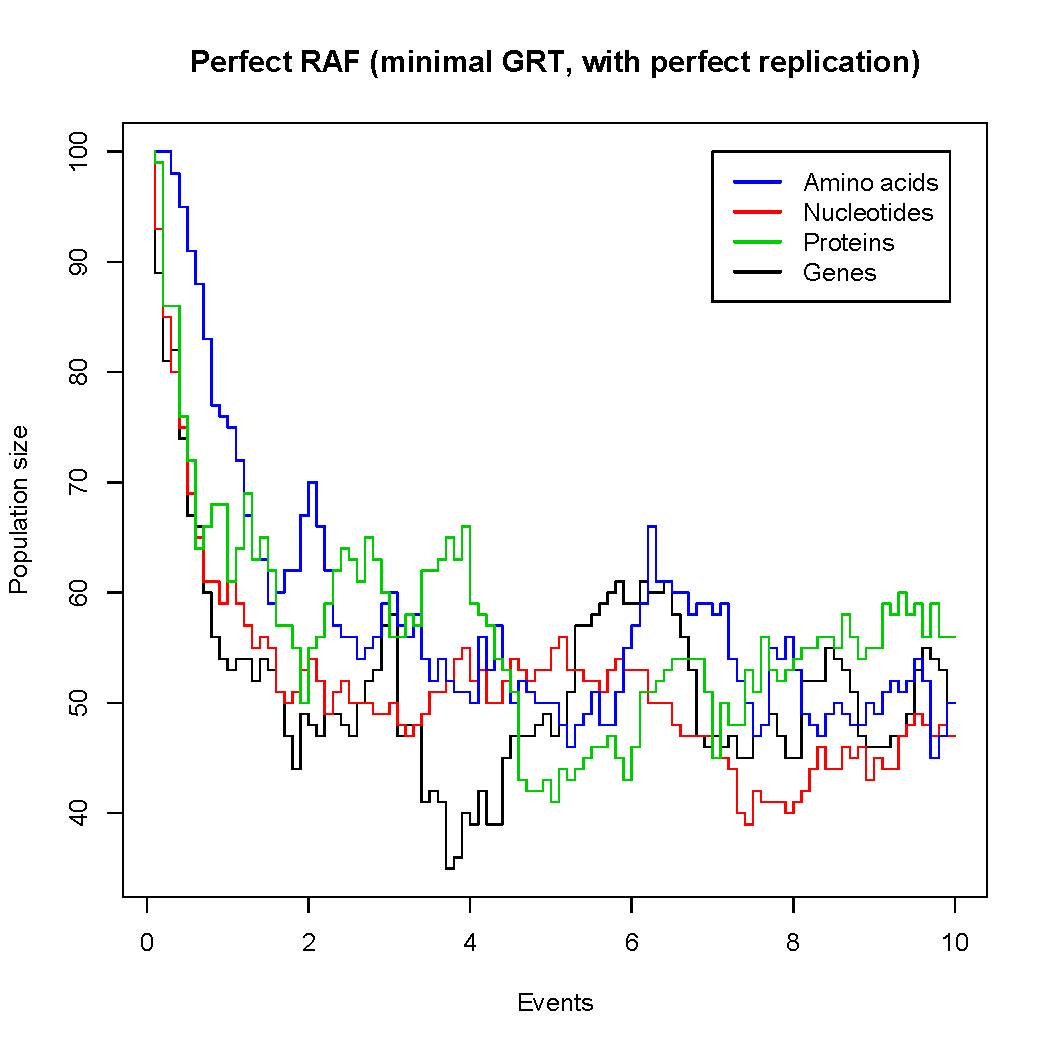
\includegraphics[width=3.5in]{PerfectRAF(minimalGRTnoError).pdf}
    \caption{(top) The simplified monopolymer model with equal initial population sizes for the food set (amino acids and nucleotides).  
    (bottom) The `perfect GRT' model with no reaction errors and with all species present in the initial conditions.}
	\label{fig:monopolymer}
\end{figure}

\begin{figure}
    \centering
    	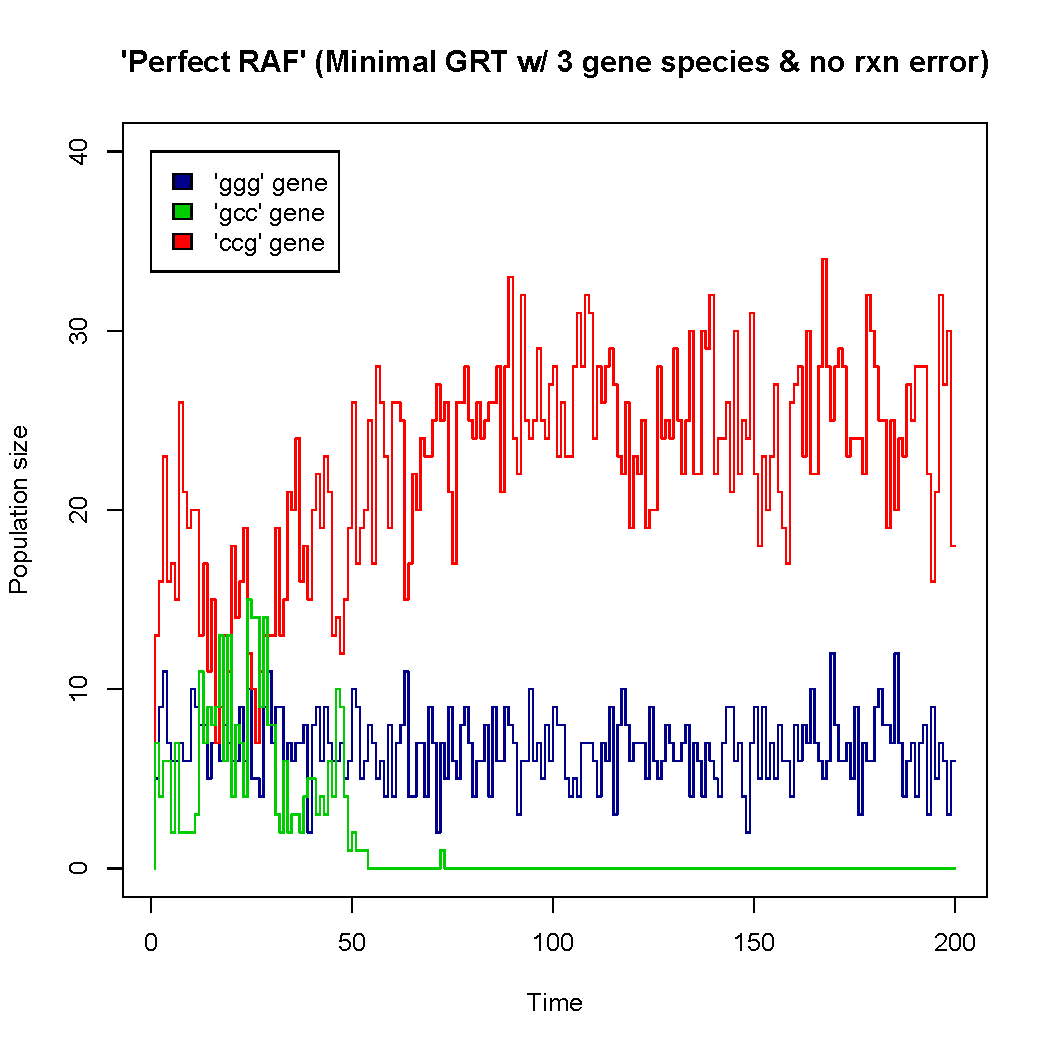
\includegraphics[width=4.5in]{PerfectRAF(minimalGRTnoError)_foodAsSpace(simTime5e4).pdf}
    \caption{The `perfect GRT' model with no reaction errors and with only the food set $F=\{g,c,a,b\}$ as part of the initial conditions, 
    (where $g$ and $c$ are nucleotides and $a$ and $b$ are amino acids).}
	\label{fig:foodAsSpace}
\end{figure}

\begin{figure}
    \centering
    	\quad
    	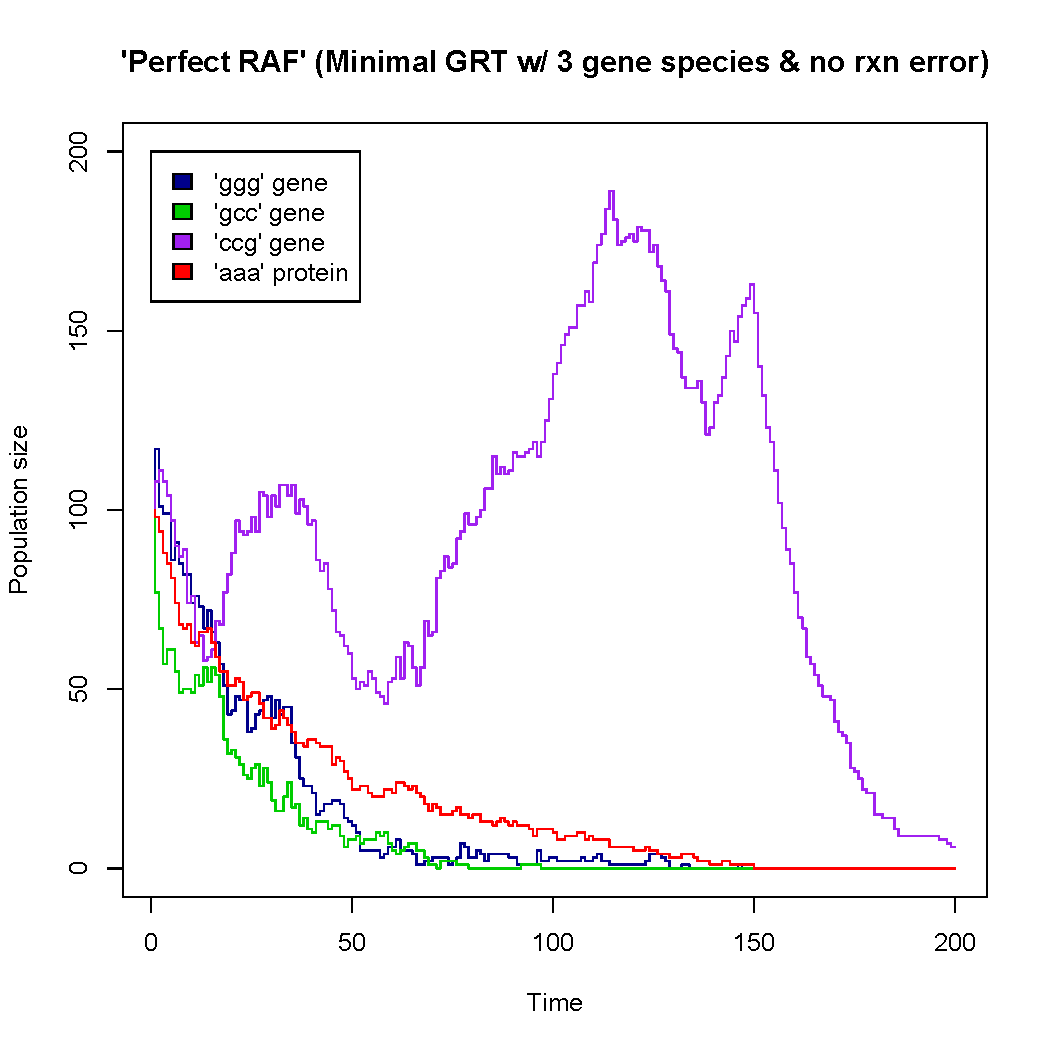
\includegraphics[width=3.5in]{PerfectRAF(minimalGRTnoError)_simTime5e3.pdf}
    	\quad
    	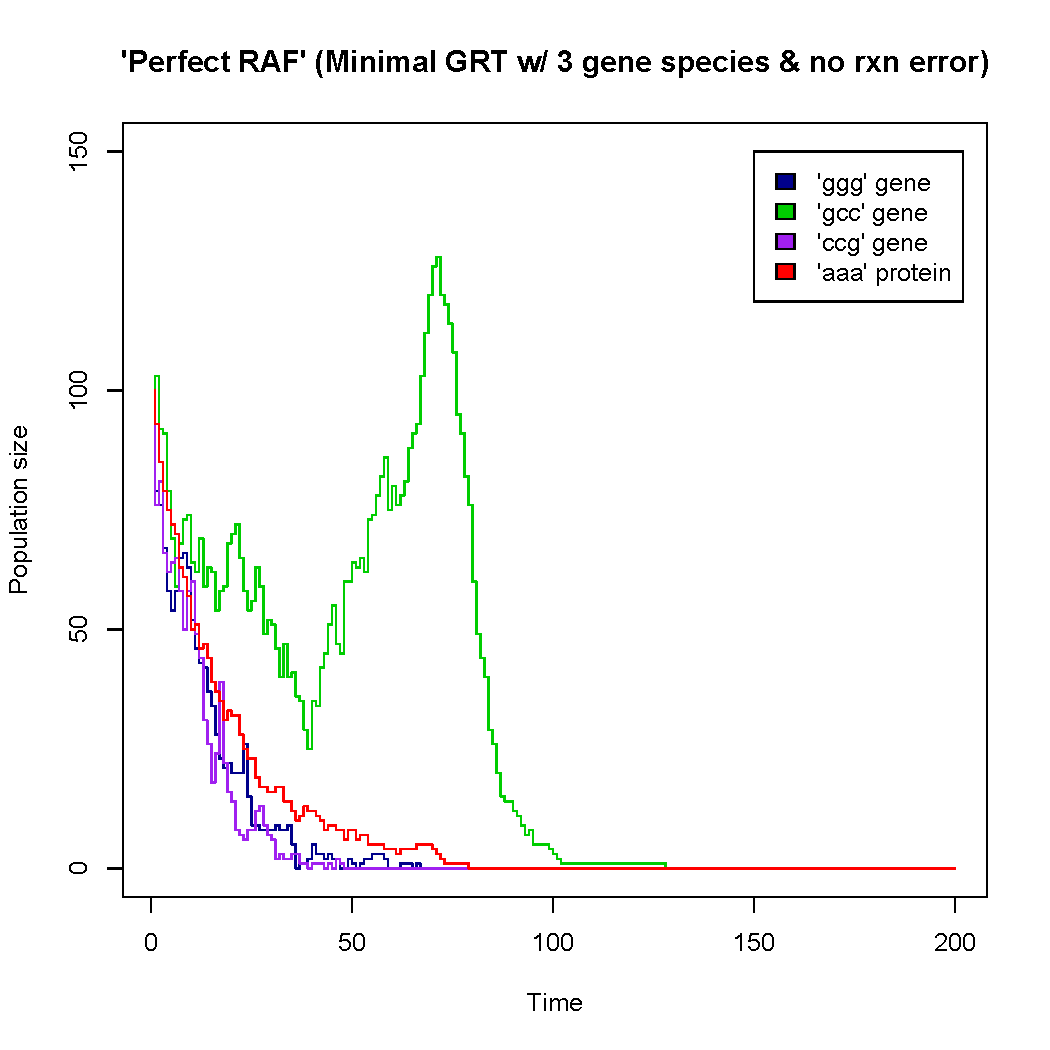
\includegraphics[width=3.5in]{PerfectRAF(minimalGRTnoError)_simTime1e4.pdf}
    \caption{(top) The `perfect GRT' model when the explicit food set was replaced with spaces $S$, with genes occupying $1S$ and proteins occupying $3S$.}
	\label{fig:spaceAsFood}
\end{figure}

\begin{figure}
    \centering
    	\quad
    	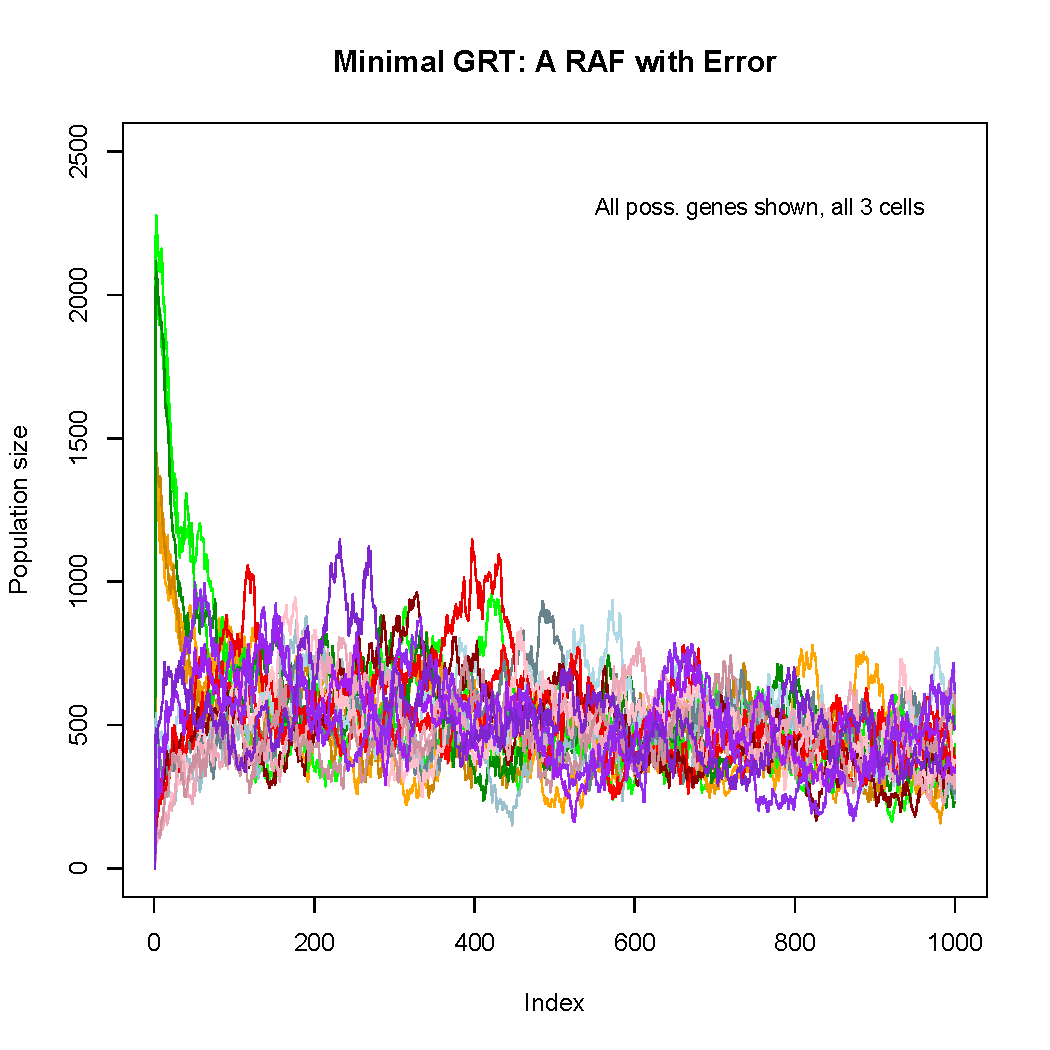
\includegraphics[width=3.5in]{MinimalGRT_RAFwithError_noDiffusion_genes.pdf}
    	\quad
    	\includegraphics[width=3.5in]{MinimalGRT_RAFwithError_noDiffusion_proteins.pdf}
    \caption{The dynamics of the gene (top) and protein (bottom) populations through time in the minimal GRT model with error in the replication and translation reactions, but no diffusion from cell to cell.}
	\label{fig:minGRTnoDiffusion}
\end{figure}

\begin{figure}
    \centering
    	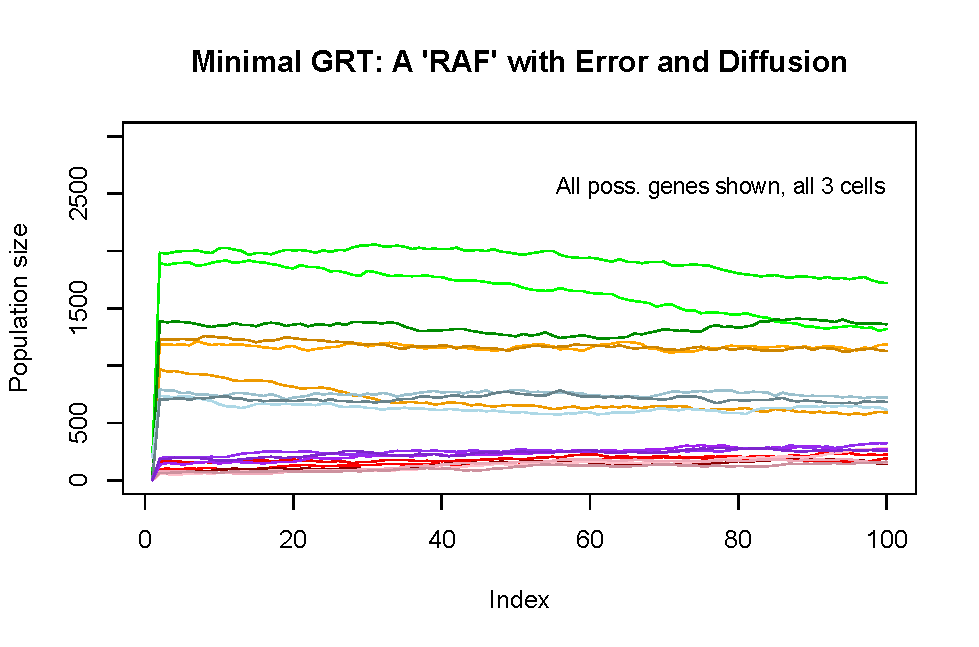
\includegraphics[width=5in]{MinimalGRT_RAFwithErrorAndDiffusion.pdf}
    \caption{The three green shades (top three) represent the replicase sequence G[0,0,0], while the orange and blue shades (the two other colours that can be seen 
    to separate themselves from the `noise') represent sequences G[0,1,1] and G[0,1,0], respectively.}
	\label{fig:minGRT}
\end{figure}


%----------------------------------------------------------------------------------------
%	BIBLIOGRAPHY
%----------------------------------------------------------------------------------------
\newpage
\begin{thebibliography}{99} % Bibliography - this is intentionally simple in this template

\bibitem[{{Des Marais \it{et al.}\/}, 2008}]{NASA}
{\sc Des Marais, D.~J.}, {\sc J.~A. Nuth III}, {\sc L.~J. Allamandola}, 
{\sc A.~P. Boss}, {\sc J.~D. Farmer}, {\sc T.~M. Hoehler}, {\sc B.~M. Jakosky}, 
{\sc V.~S. Meadows}, {\sc A. Pohorille}, {\sc B. Runnegar}, and {\sc A.~M. Spormann} 2008.
NASA Astrobiology Roadmap.
\newblock Astrobiology.

\bibitem[{{Hordijk and Steel\/}, 2004}]{Hordijk2004}
{\sc Hordijk, W.} and {\sc M. Steel} 2004. 227(4):451–61.
Detecting autocatalytic, self-sustaining sets in chemical reaction systems.
\newblock J. Theor. Biol.

\bibitem[{{Hordijk and Steel\/}, 2012a}]{Hordijk2012a}
{\sc Hordijk, W.} and {\sc M. Steel} 2012. 3:5.
Autocatalytic sets extended: dynamics, inhibition, and a generalization.
\newblock J. Syst. Chem.

\bibitem[{{Hordijk \it{et al.}\/}, 2014}]{Hordijk2014}
{\sc Hordijk, W.}, {\sc L. Hasenclever}, {\sc J. Gao}, {\sc D. Mincheva}, and {\sc J. Hein} 2014. 13:287-296.
Algorithms for detecting and analysing autocatalytic sets.
\newblock Nat. Comput.

\bibitem[{{Hordijk \it{et al.}\/}, 2015}]{Hordijk2015}
{\sc Hordijk, W.}, {\sc J.~I. Smith}, and {\sc M. Steel} 2015.
Algorithms for detecting and analysing autocatalytic sets.
\newblock Biomed Central.

\bibitem[{{Kauffman\/}, 1971}]{Kauffman1971}
{\sc Kauffman, S. A.}, 1971. 1(1):71–96. 
Cellular homeostasis, epigenesis and replication in randomly aggregated macromolecular systems.
\newblock J. Cybernet

\bibitem[{{Kauffman\/}, 1986}]{Kauffman1986}
{\sc Kauffman, S. A.}, 1986. 119:1–24.
Autocatalytic sets of proteins.
\newblock J. Theor. Biol.

\bibitem[{{Paoletti\/}, 2015}]{Paoletti}
{\sc Paoletti, F.}, 2015.
Probing prebiotic toy-chemical reaction systems for autocatalytic sets.
\newblock Report submitted to Systems Biology Doctoral Training Centre

\bibitem[{{Steel\/}, 2000}]{Steel2000}
{\sc Steel, M.}, 2000.
The emergence of a self-catalysing structure in abstract origin-of-life models.
\newblock Appl. Math. Lett.

\bibitem[{{Steel \it{et al.}\/}, 2013}]{Steel2013}
{\sc Steel, M.}, {\sc W. Hordijk}, and {\sc J. Smith}, 2013. (332)7:96-107.
The emergence of a self-catalysing structure in abstract origin-of-life models.
\newblock J. Theor. Biol.

\bibitem[{{Turing\/}, 1952}]{Turing}
{\sc Turing, A. M.}, 1952.
The chemical basis of morphogenesis.
\newblock Phil. Trans. R. Soc.

\bibitem[{{Vaughan and Drummond\/}, 2013}]{MASTER}
{\sc Vaughan, T.~G.} and {\sc A.~J. Drummond}, 2013.
A stochastic simulator of birth–death master equations with application to phylodynamics.
\newblock Mol. Biol. Evol.

\bibitem[{{Wills\/}, 2015}]{Wills2015}
{\sc Wills, P. R.}, 2015.
The generation of meaningful information in molecular systems.
\newblock Phil. Trans. R. Soc.
 
\end{thebibliography}
%----------------------------------------------------------------------------------------
\end{document}